\section[Nonlinear Boson Diffusion Equation]{Thermalization via a Nonlinear Boson Diffusion Equation}
The second part of our discussion of the thermalization process of gluons in relativistic heavy-ion collisions is based on a Nonlinear Boson Diffusion equation (NBDE) derived from the Boltzmann equation using a gradient expansion of the respective collision integral.
\subsection{Derivation of the NBDE}
Our central assumptions are spatial homogeneity of the boson distribution function $f(\mathbf{x},\mathbf{p},t)$ and spherical symmetry in the momentum dependence. These assumptions allow us to simplify the kinetic equations by performing the angular integration. We arrive at the following expression for the single-particle occupation numbers $n_j=n(\varepsilon_j,t)$ in a finite Bose system:
\begin{equation}
\begin{aligned}
\frac{\partial n_1}{\partial t} &= \sum_{\varepsilon_2,\varepsilon_3,\varepsilon_4}\langle V^{2}\rangle \cdot G(\varepsilon_1+\varepsilon_2,\varepsilon_3+\varepsilon_4)\\
&\times \left[(1+n_1)(1+n_2)n_3n_4 - (1+n_3)(1+n_4)n_1n_2\right]
\end{aligned}
\end{equation}
Here $\langle V^{2}\rangle$ is the second moment of the interaction potential and the function $G$ encodes energy conservation\footnote{For an infinite system this is simply a delta function $G(\varepsilon_1+\varepsilon_2,\varepsilon_3+\varepsilon_4)\rightarrow \pi\cdot\delta(\varepsilon_1 + \varepsilon_2 -\varepsilon_3 - \varepsilon_4)$ but in a finite system, as we want to have a look at here, the function may acquire a width due to off-shell scatterings between single-particle states which lie apart in the space of possible energies.}. The different indices $1$ to $4$ indicate the respective particles in the elastic $2\rightarrow 2$ scattering process.\\
\noindent 
The collision term on the right hand side can be rewritten in the form of a Master equation (cf. Talha's talk):
\begin{equation}
\frac{\partial n_1}{\partial t} = (1+n_1)\sum_{\varepsilon_4}W_{4\rightarrow 1}n_4	- \sum_{\varepsilon_4}W_{1\rightarrow 4}(1+n_4),	
\end{equation}
with the transition probability
\begin{equation}
W_{4\rightarrow 1}=  W_{41}g_1 = \sum_{\varepsilon_2, \varepsilon_3} \langle V^{\phantom{.}2}\rangle G(\varepsilon_1+\varepsilon_2,\varepsilon_3+\varepsilon_4)(1+n_2)n_3
\end{equation}
and $W_{1\rightarrow 4}$ analogously. Here we already introduced the density of states $g_j\equiv g(\varepsilon_j)$ which occur when taking the continuum limit. This also leads us to a replacement of the summations by integrations. Since bosons are interchangeable, $W_{14}=W_{41}$ and 
\begin{equation}
		W_{14}=W_{41}=W\left[\frac{1}{2}(\varepsilon_4+\varepsilon_1),\underbrace{\abs{\varepsilon_4-\varepsilon_1}}_{=: x}\right]
	\end{equation}
for the case of a finite system where $G$ acquires a width (cf. footnote on the last page). This means that that the transition probabilities depend only on the absolute energy difference $x$ and they are peaked around $x\simeq 0$.\\
\noindent
Performing a gradient expansion of $n_4$ and $g_4n_4$ around $x\simeq 0$ and introducing the transport coefficients
\begin{align}
	D(\varepsilon,t) = \frac{g_1}{2}\int\limits_0^{\infty}\dd x\ W(\varepsilon_1,x) \ x^2
\end{align}
and 
\begin{equation}
		v(\varepsilon,t) = g_1^{-1}\frac{d}{d\varepsilon_1}(g_1D) 
\end{equation}
via moments of the transition probability we arrive at a nonlinear partial differential equation for the number density:
\begin{equation}
			\frac{\partial n}{\partial t} = -\frac{\partial}{\partial\varepsilon}\left[v\cdot n(1+n) + n\frac{\partial n}{\partial\varepsilon}\right] + \frac{\partial^2}{\partial\varepsilon^2}\left[Dn\right]\label{eqn:nbde1}.
\end{equation}
Here $D(\varepsilon,t)$ is referred to as diffusion term and $v(\varepsilon,t)$ as drift term taking dissipative effects into account. Their explicit values are important since they define the equilibrium temperature $T$ via the relation
\begin{equation}
	T = -\frac{D}{v}.
\end{equation}
The minus sign is explained by the fact that the drift is always towards the infrared i.\,e. the low-energy regime.\\
 For our case of relativistic heavy-ion collisions it is well motivated to assume constant transport coefficients which allows us to simplify our equation to
\begin{equation}
			\frac{\partial n}{\partial t} = -v\frac{\partial}{\partial\varepsilon}\left[n(1+n)\right] + D\frac{\partial^2 n}{\partial\varepsilon^2}\label{eqn:nbde2},
		\end{equation}
with the well-known Bose-Einstein distribution		
\begin{equation}
	n_{\mathrm{eq}}(\varepsilon) = \frac{1}{\exp(\frac{\varepsilon-\mu}{T}) - 1}
\end{equation}
as a stationary solution.\\
At this point we need to discuss some general features of this model. It does not resolve the second order phase transition to the condensate discussed earlier explicitly but nevertheless the kinetics of Bose condensation before and after the transition are taken into account. After some time $t$ a certain fraction of bosons is pushed into the condensate which is a feature that may not be realized in nature. Of course it is based on particle-number conserving elastic scattering which may not provide the dominant contribution to the thermalization process as emphasized before. Another interesting feature of this certain model is that the particle number is only conserved when the integration is performed over the whole $x$-range opposed to the Boltzmann equation with energy-conserving delta function. We will see this in a moment when we analyze some plots of the solutions of the NBDE for different integration ranges. \\
To get a first analytical solution of the NBDE in the form of eqn. (\ref{eqn:nbde2}) we first want to study a linear approximation, the so-called linear relaxation ansatz (RTA).
\subsection{Linear Relaxation Ansatz}
For a given initial distribution $n_{\mathrm{t}}(\varepsilon)$  the linear relaxation-time ansatz reads 
\begin{equation}
	\frac{\partial n_{\mathrm{rel}}}{\partial t} = \frac{(n_{\mathrm{eq}} - n_{\mathrm{
rel}})}{\tau_{\mathrm{eq}}},
\end{equation}
where we introduced the equilibration time $\tau_{\mathrm{eq}} = 4D/(9v^2)$ again as a certain ratio of the transport coefficients. General solutions to this simplified model are of the form of
\begin{equation}
	n_{\mathrm{rel}}(\varepsilon,t) = n_{\mathrm{i}}(\varepsilon)\cdot\exp\left(-\frac{t}{\tau_{\mathrm{eq}}}\right) +  n_{\mathrm{eq}}(\varepsilon)\left(1-\exp\left(-\frac{t}{\tau_{\mathrm{eq}}}\right)\right).
\end{equation}
Following ref. \cite{Mueller1999} we may use an initial distribution of the subsequent form in order to concentrate on a suitable distribution in the context of heavy-ion collisions, i.\,e.
\begin{equation}
	n_{\mathrm{i}}(\varepsilon) = N_{\mathrm{i}}\cdot\theta\left(1-\varepsilon/Q_{\mathrm{s}}\right)\cdot\theta(\varepsilon) \label{eqn:rta_initial}.
\end{equation}
Here we find again the dependency on the saturation $Q_{\mathrm{s}}\simeq 1$ GeV as upper limit of the box-shaped initial gluon distribution.\\
The results for the thermalization process from the NBDE following from the RTA are displayed in figure \ref{fig:rta1} at the beginning of the next page. We observe that the thermal equilibrium is reached fast after a time of approximately $t\simeq 2\tau_{\mathrm{eq}}$ approaching the Bose-Einstein limit from above in the IR and from below in the UV. At the boundary $p\simeq Q_{\mathrm{s}}$ we encounter unphysical discontinuities. Note that here the total gluon number is set to $N_{\mathrm{i}}=1$ to facilitate the comparison with the exact analytical solutions later on. Additionally we observe that we we are again dealing with an overoccupied system since 
\begin{equation}
	N_{\mathrm{i}} = (4/3)\pi\cdot V\cdot Q_{\mathrm{s}}^3\cdot n_{\mathrm{i}}\quad >\quad N_{\mathrm{eq}} = 4\pi\cdot V \int_0^{\infty} n_{\mathrm{eq}}\cdot\varepsilon^2\ \dd\varepsilon
\end{equation}
If we would assume overall particle number conservation we would come again to the conclusion that the excess particles are driven into a condensate such that not only the gluon number in the thermal spectrum but rather the sum of the thermal gluons and the ones in the condensate is conserved.


\begin{figure}[t]
\centering
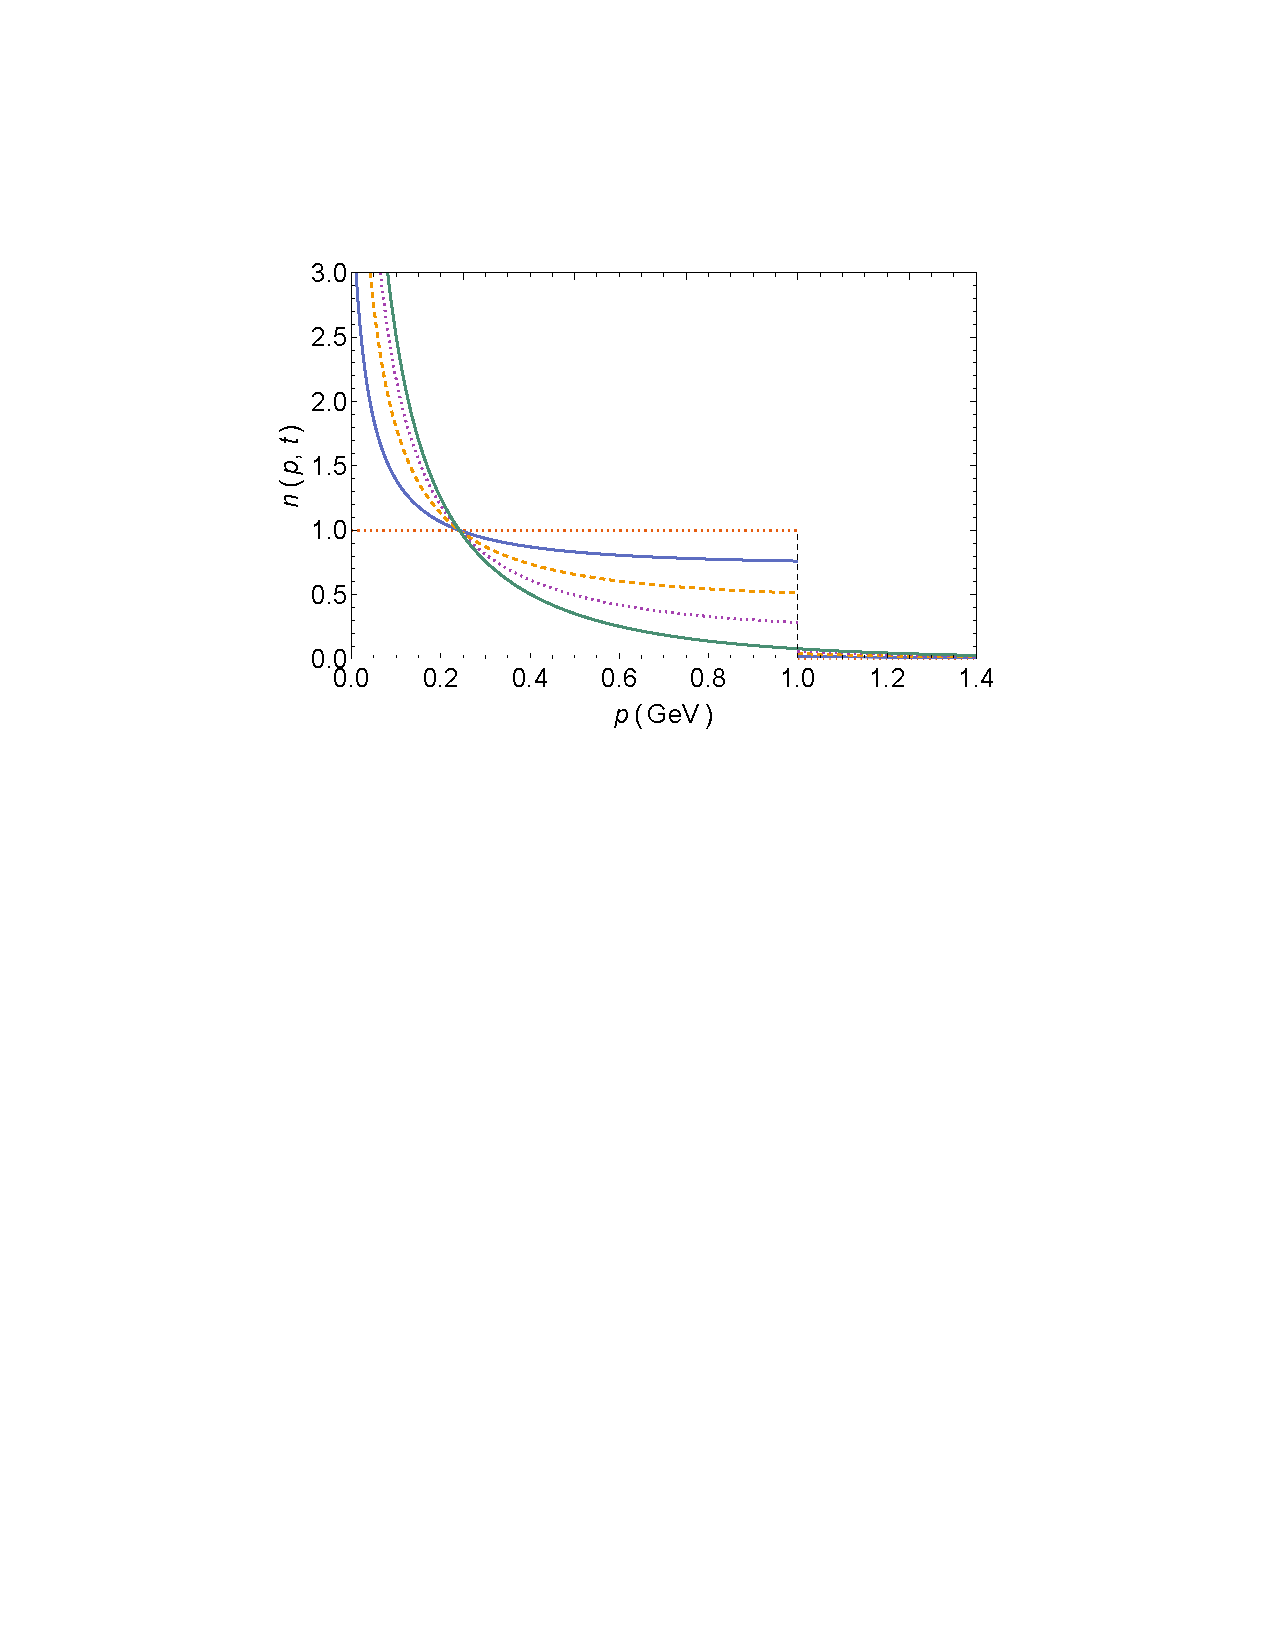
\includegraphics[width = 0.7\textwidth]{figures/rta}
\caption{Linear relaxation of a finite Bose system towards the equilibrium \cite{Wolschin2018}. \\ Here $T = -D/v \simeq 0.4\ \mathrm{GeV}$, $\tau_{\mathrm{eq}} = 4D/(9v^2) = 0.33\cdot 10^{-23} \mathrm{s} \simeq 1\ \mathrm{fm/c}$ and the timesteps are $\left\{0.1, 0.25, 0.5,\infty\right\}$ (in units of $10^{-23}s$) from top to bottom.} 
\label{fig:rta1}
\end{figure}


\subsection{Exact solution of the NBDE}
To be able to find a solution to the full NBDE we perform the nonlinear transformation\footnote{Another possible solution is given by Burger's equation $\frac{\partial w}{\partial t} + w\frac{\partial w}{\partial\varepsilon} = D\frac{\partial^2 w}{\partial\varepsilon^2}$ following from the linear transformation $n(\varepsilon,t) = \frac{1}{2v}w(\varepsilon,t) - \frac{1}{2}$ but we will not discuss the details of this approach here.} 
\begin{equation}
		n(\varepsilon,t) = -\frac{D}{v}\frac{\partial \ln \mathcal{Z}(\varepsilon,t)}{\partial\varepsilon}
\end{equation}
with the usual partition sum $ \mathcal{Z}(\varepsilon,t)$ reducing our problem to a linear diffusion equation for the partial sum, i.\,e.
\begin{equation}
		\frac{\partial  \mathcal{Z}}{\partial t} = -v\frac{\partial  \mathcal{Z}}{\partial \varepsilon} +  D\frac{\partial^2  \mathcal{Z}}{\partial \varepsilon^2}.
	\end{equation}
General solutions of the NBDE are then of the form 	
\begin{equation}
n(\varepsilon, t)=\frac{1}{2 v} \frac{\int_{-\infty}^{+\infty} \frac{\varepsilon-x}{t} F(x)\cdot G_{\mathrm{free}}(\varepsilon-x,t)\ \dd x}{\int_{-\infty}^{+\infty} F(x)\cdot G_{\mathrm{free}}(\varepsilon-x,t)\ \dd x}-\frac{1}{2},
\end{equation}
with the free Green's function, being an usual Gaussian,
\begin{align}
	G_{\mathrm{free}}(\varepsilon-x,t) = \exp\left[-\frac{(\varepsilon-x)^2}{4Dt}\right],
\end{align}
and the function $F(x)$ taking the initial conditions into account, i.\,e.
\begin{equation}
	    F(x)  = \exp\left[-\frac{1}{2D}(vx+2v\int_0^x n_{\mathrm{i}}(y) \dd y) \right].
\end{equation}
They define the partition sum via the relation
\begin{equation}
	\mathcal{Z}(\varepsilon,t) = a(t)\cdot\int_{-\infty}^{\infty} G_{\mathrm{free}}(\varepsilon,x,t)\cdot F(x)\ \dd x,
\end{equation}
with some energy-independent scaling factor $a(t)$ which is in our case not important since it drops out due to the $\operatorname{log}$-derivative. As already mentioned before one may check that the particle number is not conserved for an integration over only the positive $x$-range. With these definitions in mind we are now set to present the results of the NBDE. At this point I should mention that I will not display the full lengthy expressions for the full analytical solution but rather focus on the plots and the implications arising from these different solutions. In case the reader may be interested in the exact expressions I refer to ref. \cite{Wolschin2018} for the first part and to ref. \cite{Wolschin2020_1} for the second part.
\begin{figure}[H]
\begin{subfigure}[c]{0.49\textwidth}
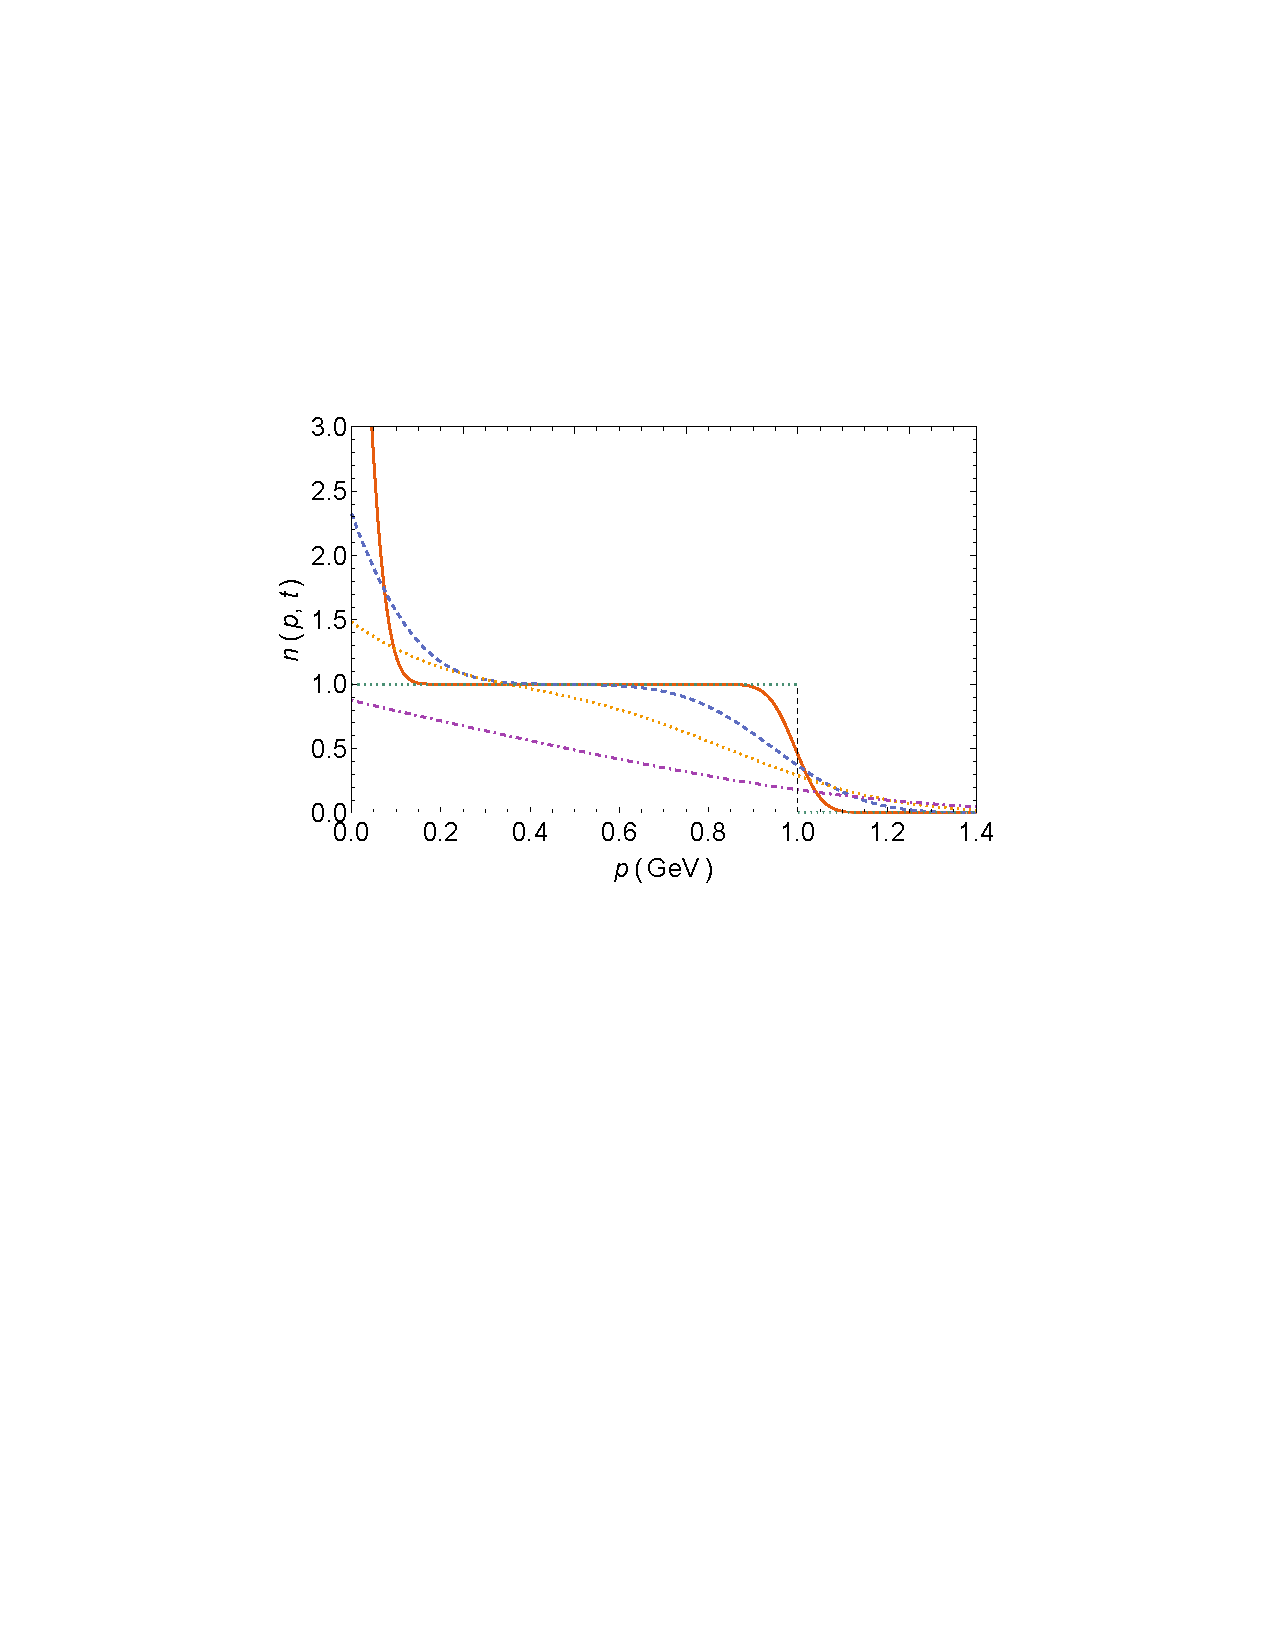
\includegraphics[width=\textwidth]{figures/nbde_positive_range}
\subcaption{Integration range restricted to $x \geq 0$.\\ The timesteps are $\left\{0.005, 0.05, 0.15,0.5\right\}$ \\ (in units of $10^{-23}s$) from top to bottom.}
\end{subfigure}
\begin{subfigure}[c]{0.49\textwidth}
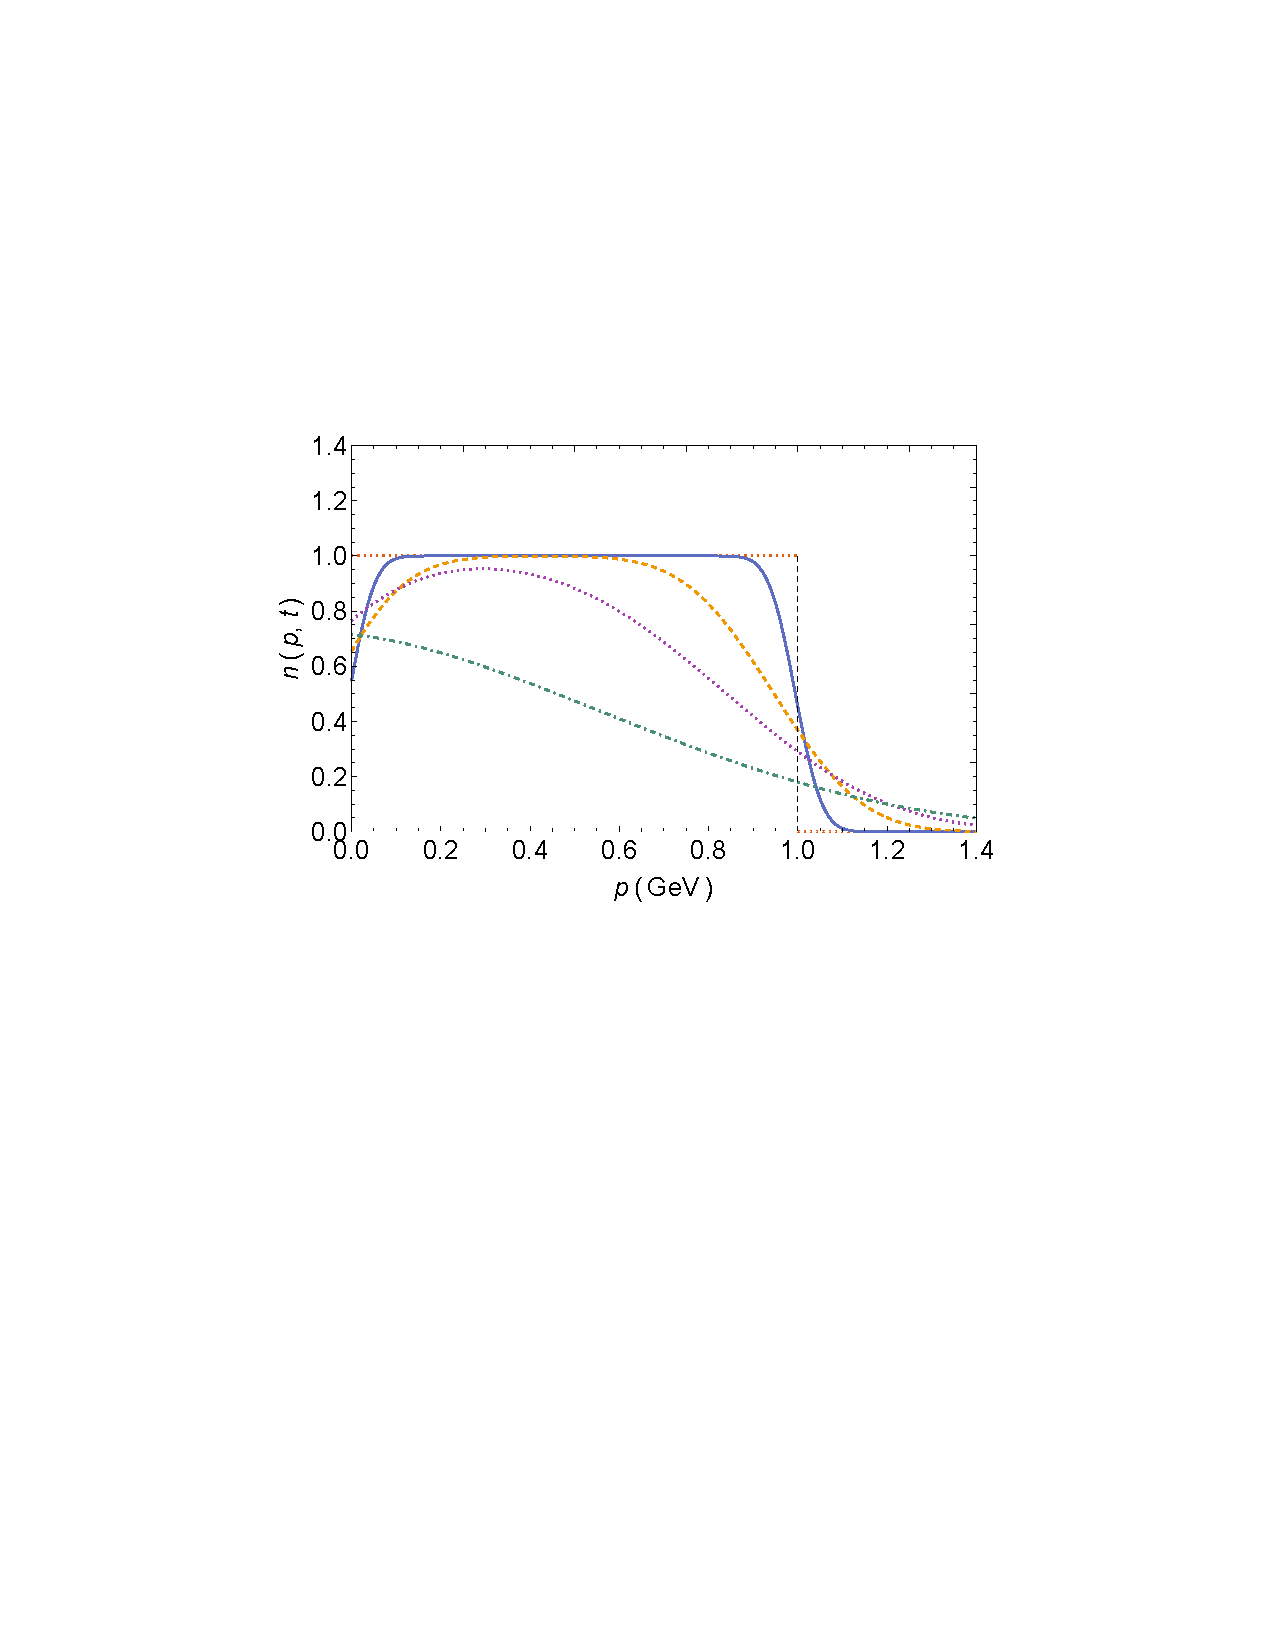
\includegraphics[width=\textwidth]{figures/nbde_full_range}
\subcaption{Integration range extended to $-\infty \leq x \leq \infty$. \\ The timesteps are $\left\{0.005, 0.05, 0.15,0.5\right\}$ \\ (in units of $10^{-23}s$) from top to bottom.}
\end{subfigure}
\caption{Equilibration of a finite Bose system from the NBDE for $T\simeq 0.4\ \mathrm{GeV}$ and \\ $\tau_{\mathrm{eq}} =  0.33\cdot 10^{-23} \mathrm{s}$ \cite{Wolschin2018}.}
\label{fig:full_sol_ranges}
\end{figure}
\noindent
In the above figure \ref{fig:full_sol_ranges} we present the results for the equilibration following from the exact solutions for different integration ranges to highlight the importance of integrating over the whole $x$-range. In the left figure we find the occupation rising above the thermal limit for very short times but due to redistribution into the condensate it depletes and we have $n(0,t)<1 \ \forall t >\tau_{\mathrm{eq}}$ which encodes the explicit violation of particle number conservation. In the right plot, representing the solution with integration over the whole range, we directly see the redistribution into the condensate in the IR already at early times and find a new thermal tail developed in the UV. We therefore conclude that these solutions do not reproduce the expected features of the Bose-Einstein equilibrium distribution, yet. This can be explained by the fact that we did not yet include  the singularity of the Bose-Einstein distribution at $\varepsilon=\mu <0$. We will see how to resolve this problem in the following.

\subsection{Including the Singularity}
To account for the singularity at $\varepsilon=\mu <0$ we have to modify the initial distribution (\ref{eqn:rta_initial}) in the following way:
\begin{equation}
		\tilde{n_{\mathrm{i}}}(\varepsilon) = n_{\mathrm{i}}(\varepsilon) + \frac{1}{\exp\left(\frac{\varepsilon-\mu}{T}\right)-1}.
	\end{equation}
For the subsequent analysis we treat the chemical potential $\mu$ as a fixed parameter and consider the asymptotics of 	our distribution at the singularity
\begin{equation}
	 \lim_{\varepsilon\rightarrow\mu^{+}}\ n(\varepsilon,t) = \infty\ \forall t 
\end{equation} 
yielding $\mathcal{Z}(\mu,t) = 0$. This results in a modified expression for the Green's function 
 	\begin{equation}
		G(\varepsilon,x,t) = G_{\mathrm{free}}(\varepsilon-\mu,x,t) - G_{\mathrm{free}}(\varepsilon-\mu,-x,t).
\end{equation}
This means that in general our expressions for the partition sum and the function $F$ stay almost the same except in a shift in the respective argument by the chemical potential $\mu$. The techniques to solve the NBDE with this boundary condition remain the same and we can therefore have a look at the solutions displayed below in figure (\ref{fig:singularity}).
\begin{figure}[H]
\begin{subfigure}[c]{0.47\textwidth}
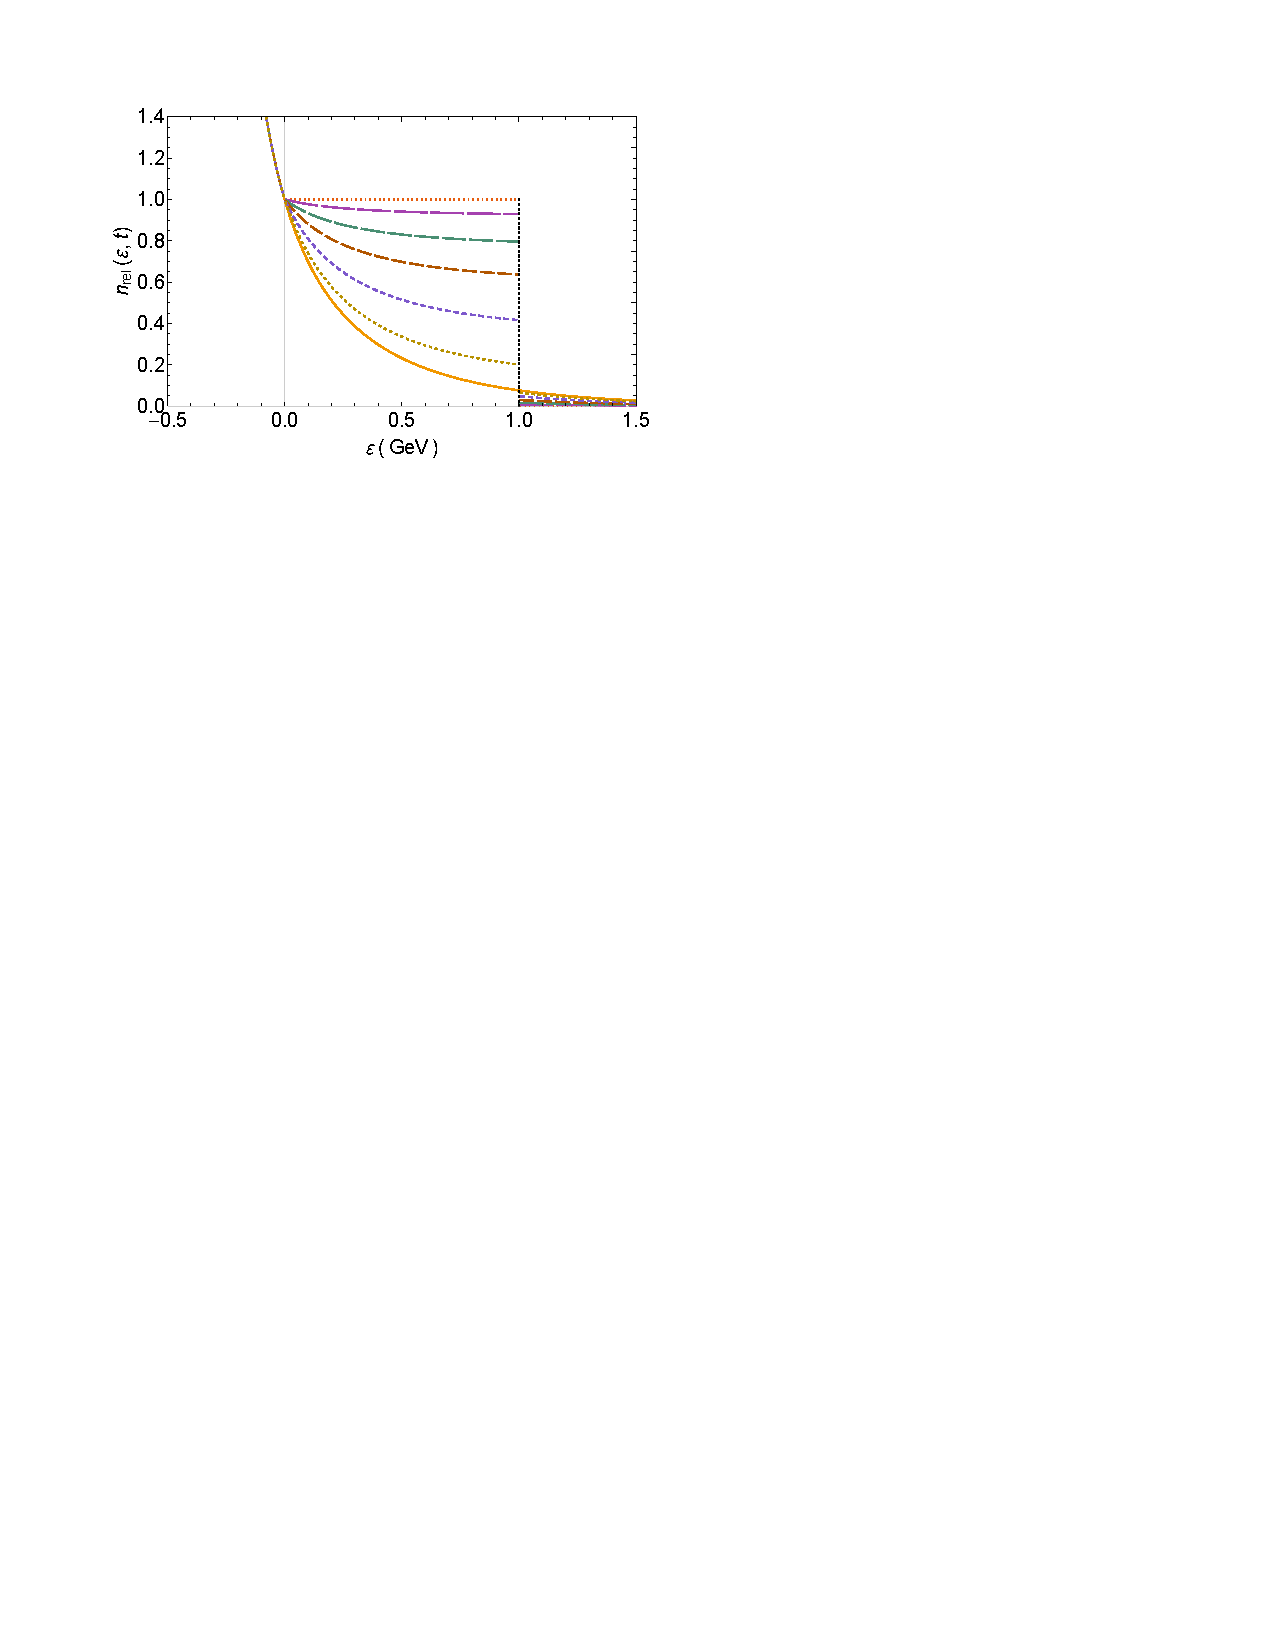
\includegraphics[width=\textwidth]{figures/rta_full}
\subcaption{Local thermalization of gluons in the linear RTA.
The timesteps are $\left\{0.02, 0.08, 0.15,0.3,0.6\right\}$ ($\mathrm{fm}/c$) for decreasing dash length.}
\end{subfigure}
\begin{subfigure}[c]{0.495\textwidth}
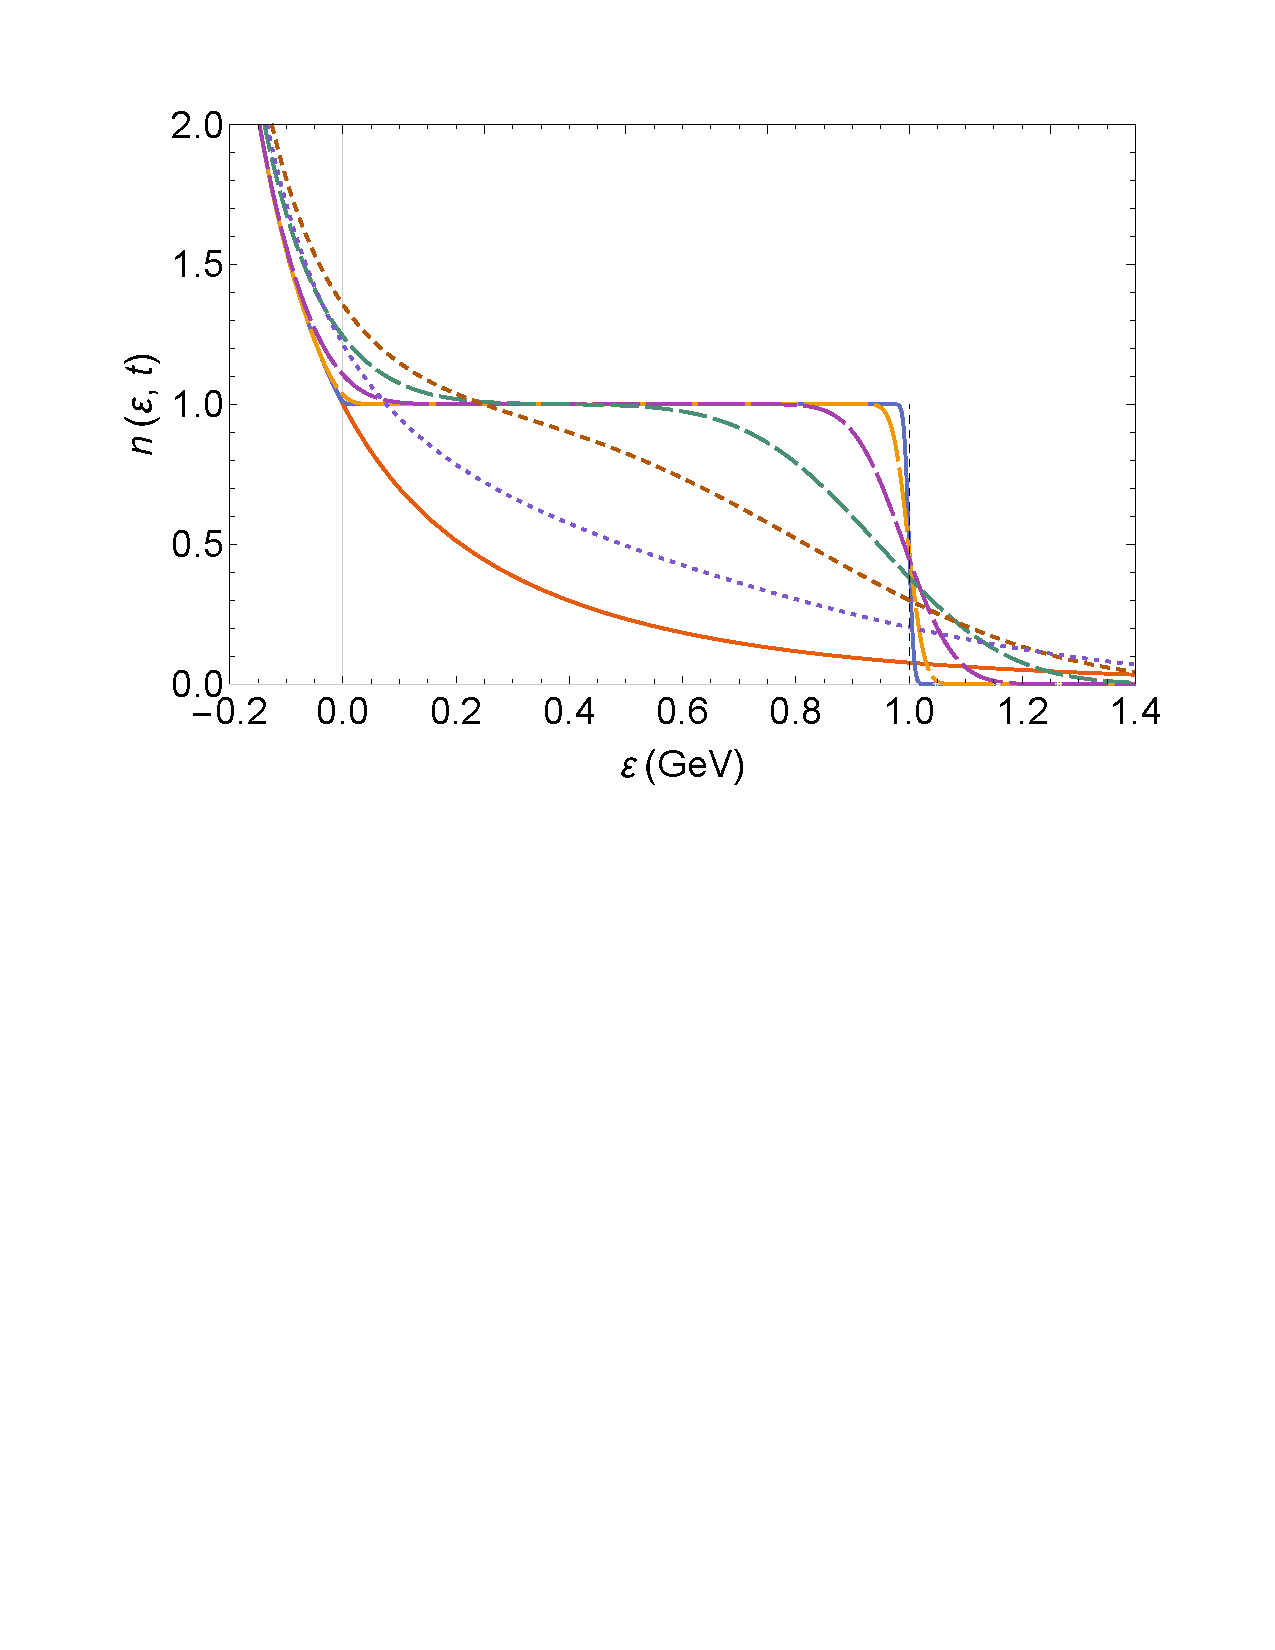
\includegraphics[width=\textwidth]{figures/nbde_full_result}
\subcaption{Local thermalization of gluons from the time-dependent solutions of the NBDE.\\ Here $\left\{6\cdot10^{-5}, 6\cdot10^{-4}, 6\cdot10^{-3},0.12,0.36\right\}$ ($\mathrm{fm}/c$) for decreasing dash length.}
\end{subfigure}
\caption{Results for the full solution of the NBDE including the singularity at $\varepsilon=\mu<0$ at $T \simeq 513\ \mathrm{MeV}$ \cite{Wolschin2020_1}. }
\label{fig:singularity}
\end{figure}
\noindent
In the left figure we see again the simplified solution arising from the RTA where we can already observe that the solution entails the correct physical properties of the Bose-Einstein equilibrium distribution in the UV and finally also in the IR except the discontinuities at $p\simeq Q_{\mathrm{s}}$. Note that here the thermalization occurs much slower than in the nonlinear case on the right hand side.\\
\noindent
The full nonlinear solution presented in the right figure now appropriately describes the thermalization process of a finite gluon system encoding all expected properties in the UV and also in the IR opposed to the first solutions omitting the important boundary condition at $\varepsilon=\mu$. Note that in our concrete example the numerical values of the transport coefficients have been chosen such that they represent the situation of a Pb-Pb collision at the LHC with a center-of-mass energy of $\sqrt{s}=5$ TeV leading to a thermalization with $T\simeq 513$ MeV.